\section{Qualità di prodotto}
La qualità di un prodotto software è valutata secondo criteri semplici e comprensibili a tutti, utenti e sviluppatori, operatori e addetti alla manutenzione.
Per valutare tale qualità il gruppo \Gruppo ha deciso di far riferimento allo standard ISO/IEC 9126, le quali norme descrivono:
\begin{itemize}
\item un modello di qualità del software; 
\item le caratteristiche che determinano la qualità del software;
\item le metriche per la misurazione della qualità del software.
\end{itemize}

\begin{figure}[h]
    \centering
    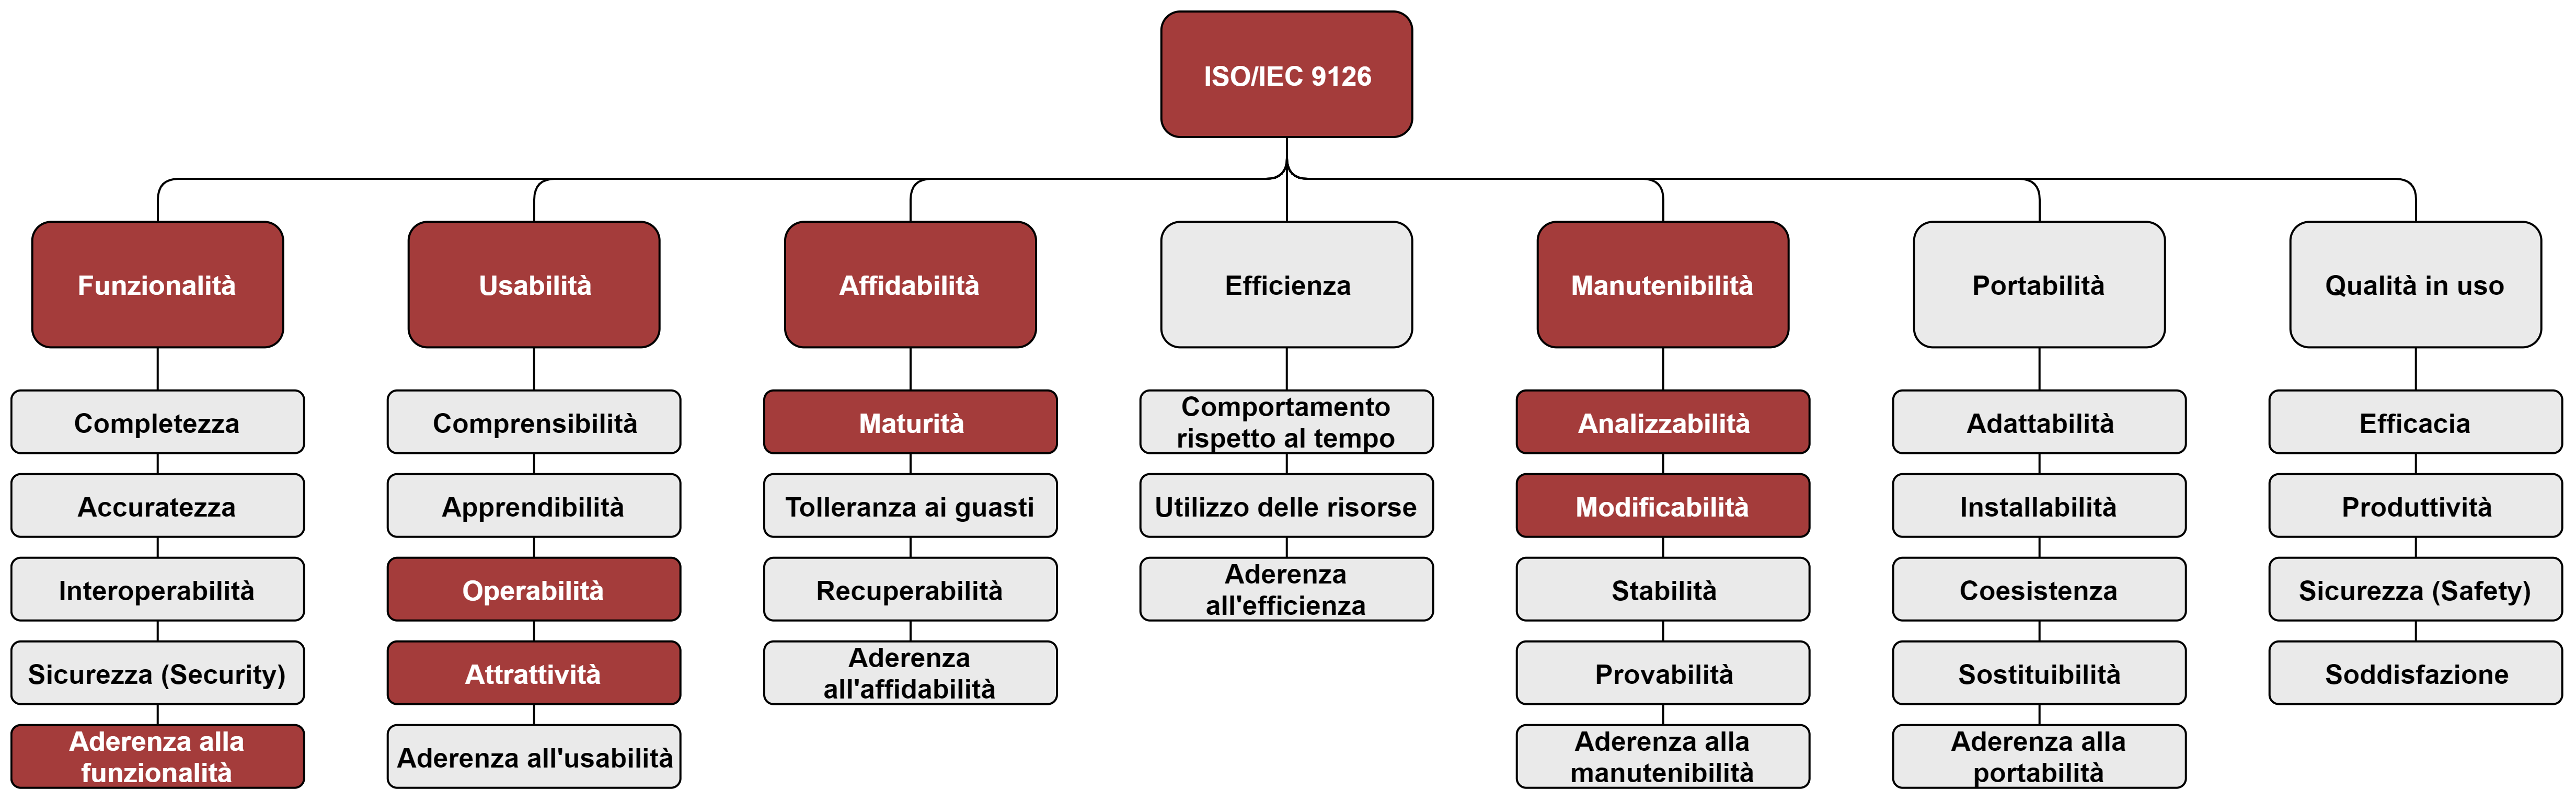
\includegraphics[scale=0.53]{sezioni/Immagini/Iso_Iec_9126.png}
    \caption{Schema dello standard ISO/IEC 9126. In rosso sono indicate le caratteristiche e attributi di interesse per il progetto.}
\end{figure}

\textbf{Metriche della qualità del prodotto:}
Il modello di qualità del software descritto dalle norme ISO/IEC 9126 definisce le caratteristiche e sottocaratteristiche del software, ciascuna misurabile da metriche interne o esterne.
Una volta specificati i requisiti di qualità del prodotto software, si identificano le caratteristiche e sottocaratteristiche di qualità che più contribuiscono ad indirizzare i requisiti elencati.\\
Il gruppo \Gruppo si è impegnato a scegliere le metriche interne che maggiormente influenzano le caratteristiche esterne del prodotto finale, in modo che esse possano predire quanto più possibile il risultato finale.\\
In questa sezione di documento verranno riportate solo alcune delle caratteristiche definite dallo standard, ovvero quelle ritenute più inerenti ai fini del progetto.

\subsection{Metriche interne}
 Le metriche della qualità "interne" del software sono utilizzate durante la fase di sviluppo e permettono di valutare il comportamento del software dal punto di vista degli sviluppatori e di predire quello che sarà il punto di vista esterno degli utenti.
  \subsubsection{Funzionalità}
      Capacità del prodotto software di soddisfare i requisiti funzionali e le necessità degli utenti.

              \paragraph{Metrica - Aderenza delle funzioni e/o delle interfacce} 
              \begin{itemize}
          \item  \textbf{Codice:} MPD-01
        \item    \textbf{Descrizione:} Misurare in percentuale il livello di aderenza delle funzioni e delle interfacce sviluppate rispetto agli standard, alle normative e alla regolamentazioni.
          \item  \textbf{Attributo di riferimento:} Aderenza alle funzionalità 
        \item    \textbf{Sigla:} $AFI$
         \item   \textbf{Formula:} $$AFI = {A \over B}$$
                con:
                \begin{itemize}
                    \item  $A$ = numero di funzioni(e/o interfacce) sviluppate che risultano aderenti a standard, regole e normative emesse al riguardo
                    \item  $B$ = numero totale di funzioni(e/o interfacce) che devono essere aderenti a tali regole come descritto nelle specifiche
                \end{itemize}

                \item \textbf{Range di valori che può assumere:}
                \begin{itemize}
                    \item \textbf{Accettabile:} $AFI = \geq80\% $
                    \item \textbf{Ottimale:} $AFI = 100\%$
                \end{itemize}
            \end{itemize}
              
  \subsubsection{Affidabilità} 
  Capacità di predire se il prodotto software in questione potrà soddisfare i requisiti prescritti per l'affidabilità dal punto di vista degli sviluppatori.
        \paragraph{Metrica - Rilevamento dei difetti} 
                \begin{itemize}
        \item   \textbf{Codice:} MPD-02
        \item   \textbf{Descrizione:} Misurare in percentuale l'efficacia nel rilevare i difetti presenti nel software durante lo sviluppo del prodotto.
    \item    \textbf{Attributo di riferimento:} Maturità
    \item    \textbf{Sigla:} $RD$
    \item    \textbf{Formula:} $$RD = {A \over B}$$
            con:
            \begin{itemize}
                \item $A$ = numero di difetti rilevati nelle revisioni tecniche, ispezioni e test del prodotto durante lo sviluppo
                \item $B$ = numero totale di difetti previsti durante lo sviluppo
            \end{itemize}
             
             \item \textbf{Range di valori che può assumere:}
        \begin{itemize}
            \item \textbf{Accettabile:} $RD = \geq80\% $
            \item \textbf{Ottimale:} $RD = 100\%$
        \end{itemize}
       \end{itemize}
              
      
\subsubsection{Usabilità} 
Capacità del prodotto software di essere comprensibile, di poter essere usato e compreso facilmente, in ogni sua parte, da qualsiasi utente che lo voglia usare. \\

	 \paragraph{Metrica - Validità dei dati d'input} 
	    \begin{itemize}
          \item  \textbf{Codice: } MPD-03
           \item \textbf{Descrizione:} Misurare il livello di correttezza dei dati forniti in input all'applicazione.
         \item   \textbf{Attributo di riferimento:} Operabilità
          \item  \textbf{Sigla:} $VDI$
         \item   \textbf{Formula:} $$VDI = {A \over B}$$
            con:
            \begin{itemize}
                \item $A$ = numero dei dati di input di cui si effettua il controllo di validità 
                \item $B$ = numero totale di dati di input previsti
            \end{itemize}
             
        \item \textbf{Range di valori che può assumere:}
        \begin{itemize}
            \item \textbf{Accettabile:} $VDI = $
            \item \textbf{Ottimale:} $VDI = $
        \end{itemize}
       \end{itemize}
              
                
    \paragraph{Metrica - Attrattività delle interfacce utente} 
        \begin{itemize}
          \item  \textbf{Codice: } MPD-04
          \item  \textbf{Descrizione:} Misurare quanto attrattive risultino le interfacce agli utenti dal punto di vista grafico. Gli utenti dovranno poi compilare 
          un questionario in base all'esperienza che hanno fatto. Il valore medio di tale valutazione è ritenuto valido se almeno tre utenti hanno compilato il questionario. 
          Viene utilizzata una scala a quattro valori: Molto attrattivo, Attrattivo, Poco attrattivo, Non Attrattivo.
          \item  \textbf{Attributo di riferimento:} Attrattività
          \item  \textbf{Sigla:} $AIU$
           \item \textbf{Formula:}$$AIU = V (q) $$
           con:
        \begin{itemize}
            \item $V$ = Valore medio dei risultati
            \item $q$ = Questionario compilato
        \end{itemize}

        \item \textbf{Range di valori che può assumere:}
        \begin{itemize}
            \item \textbf{Accettabile:} $AIU = Attrattivo$ 
            \item \textbf{Ottimale:} $AIU = Molto \; attrattivo$
        \end{itemize}
    \end{itemize}


        \subsubsection{Manutenibilità} 
    Capacità di predire il livello di impegno richiesto per modificare il prodotto software dal punto di vista degli sviluppatori.
    
        \paragraph{Metrica - Diagnostica} 
           \begin{itemize}
          \item  \textbf{Codice:} MPD-05
          \item  \textbf{Descrizione:} Misurare in percentuale il livello di diagnostica che il prodotto consente tramite le apposite funzioni.
          \item  \textbf{Attributo di riferimento:} Analizzabilità
         \item   \textbf{Sigla:} $D$
          \item  \textbf{Formula:} $$D = {A \over B}$$
          con:
          \begin{itemize}
            \item $A$ = numero di funzioni di diagnostica sviluppate
            \item $B$ = numero totale di funzioni di diagnostica previste nelle specifiche
          \end{itemize}

        \item \textbf{Range di valori che può assumere:}
        \begin{itemize}
            \item \textbf{Accettabile:} $D = \geq80\% $
            \item \textbf{Ottimale:} $D = 100\% $
        \end{itemize}
       \end{itemize}
              
\newpage %adattamento pagina pdf

           \paragraph{Metrica - Complessità del software} 
              \begin{itemize}
         \item   \textbf{Codice:} MPD-06
         \item   \textbf{Descrizione:} Misurare la complessità ciclomatica dei singoli moduli sviluppati.
          \item  \textbf{Attributo di riferimento:} Modificabilità
          \item  \textbf{Sigla:} $CS$
         \item   \textbf{Formula:} $$CS = v(G) = e - n + p $$
         con:
         \begin{itemize}
            \item $G$ = grafo del modulo
            \item $e$ = numero di congiunzione tra statement corrispondenti agli archi di un grafo
            \item $n$ = numero di nodi presenti nel grafo
            \item $p$ = numero delle componenti connesse da ogni arco (per esecuzione sequenziale: p=2, essendovi un predecessore e un successore)
         \end{itemize}
           
        \item \textbf{Range di valori che può assumere:}
        \begin{itemize}
            \item \textbf{Accettabile:} $1\leq CS \geq7 $
            \item \textbf{Ottimale:} $ 1\leq CS \geq4 $
        \end{itemize}
       \end{itemize}
              

\paragraph{Metrica - Unità documentate} 
   \begin{itemize}
          \item  \textbf{Codice:} MPD-07
         \item   \textbf{Descrizione:} Misurare in percentuale il numero di unità di codice con documentazione tecnica.
         \item   \textbf{Attributo di riferimento:} Modificabilità
         \item   \textbf{Sigla:} $RM$
         \item   \textbf{Formula:} $$RM = {A \over B}$$
         con:
         \begin{itemize}
            \item $A$ = numero di unità di codice con documentazione tecnica inserita 
            \item $B$ = numero totale di unità di codice
                     \end{itemize}

        \item \textbf{Range di valori che può assumere:}
        \begin{itemize}
            \item \textbf{Accettabile:} $RM = \geq90\%  $
            \item \textbf{Ottimale:} $RM = 100\%$
        \end{itemize}
       \end{itemize}
              
       
\subsection{Metriche esterne}
Le metriche relative alla qualità "esterna" indirizzano le caratteristiche esteriori del software, cioè quelle rilevabili direttamente dagli utenti e dagli operatori.
   \subsubsection{Funzionalità}
   Capacità del prodotto software di fornire funzioni adeguate al contesto di applicazione.
   
    \paragraph{Metrica - Completezza delle funzionalità sviluppate} 
        \begin{itemize}
        \item  \textbf{Codice:} MPD-08
        \item  \textbf{Descrizione:} Misurare il livello di completezza delle funzioni sviluppate.
        \item  \textbf{Attributo di riferimento:} Adeguatezza
        \item  \textbf{Sigla:} $CFS$
        \item  \textbf{Formula:} $$CFS = 1 - {A \over B}$$
        con:
        \begin{itemize}
            \item $A$ = numero di funzioni omesse
            \item $B$ = numero totale di funzioni previste nelle specifiche       
        \end{itemize}

        \item \textbf{Range di valori che può assumere:}
        \begin{itemize}
            \item \textbf{Accettabile:} $CFS = $
            \item \textbf{Ottimale:} $CFS = $
        \end{itemize}
    \end{itemize}
              
\subsubsection{Affidabilità}
   Capacità del prodotto software di dimostrare un adeguato livello di affidabilità quando opererà nel sistema in cui è previsto debba operare.
       
    \paragraph{Metrica - Maturità dei test} 
        \begin{itemize}
        \item   \textbf{Codice:} MPD-09
        \item  \textbf{Descrizione:} Misurare la percentuale di casi di test eseguiti con successo rispetto al numero totale previsto per garantire piena copertura dei requisiti sia funzionali che qualitativi(usabilità, affidabilità, efficienza).
        \item   \textbf{Attributo di riferimento:} Maturità
        \item    \textbf{Sigla:} $MT$
        \item   \textbf{Formula:} $$MT = {A \over B}$$
        con:
        \begin{itemize}
            \item $A$ = numero di casi di test eseguiti con successo
            \item $B$ = numero totale di casi di test previsto
        \end{itemize}
        
        \item \textbf{Range di valori che può assumere:}
        \begin{itemize}
            \item \textbf{Accettabile:} $MT = 100\% $
            \item \textbf{Ottimale:} $MT = 100\% $
        \end{itemize}
    \end{itemize}
       
\subsubsection{Usabilità}
   Capacità del prodotto software di essere facilmente comprensibile, apprendibile ed operabile per ogni utente intenzionato a usarlo.
   
    \paragraph{Metrica - Completezza della descrizione funzionale} 
        \begin{itemize}
            \item   \textbf{Codice:} MPD-10
            \item   \textbf{Descrizione:} Misurare la percentuale di funzioni comprese dall'utente dopo aver letto la descrizione del prodotto(es. Manuale utente, specifiche funzionali).
            \item    \textbf{Attributo di riferimento:} Accuratezza
            \item   \textbf{Sigla:} $CDF$
            \item   \textbf{Formula:} $$CDF = {A \over B}$$
            con:
            \begin{itemize}
            \item  $A$ = numero di funzioni comprese
            \item  $B$ = numero totale di funzioni disponibili
            \end{itemize}

            \item \textbf{Range di valori che può assumere:}
            \begin{itemize}
                \item \textbf{Accettabile:} $CDF = 70\% $
                \item \textbf{Ottimale:} $CDF = 100\% $
            \end{itemize}
        \end{itemize}

    \paragraph{Metrica - Profondità strutturale dell'applicazione}
    \begin{itemize}
        \item \textbf{Codice:} MPD-11
        \item \textbf{Descrizione:} È sconsigliato per le applicazioni l'utilizzo di una struttura troppo profonda per questioni di usabilità. L'utente non deve fare troppi passaggi per raggiungere la funzionalità desiderata. 
        \item \textbf{Attributo di riferimento:} Operabilità
        \item \textbf{Sigla:} $PSA$
        \item \textbf{Range di valori che può assumere:}
        \begin{itemize}
            \item \textbf{Accettabile:} $1 \leq PSA \leq 4$
            \item \textbf{Ottimale:} $1 \leq PSA \leq 2$
        \end{itemize}
    \end{itemize}

\subsection{Tabella metriche interne del prodotto}
    \rowcolors{2}{grigetto}{white}
    \renewcommand{\arraystretch}{1.5}
    \begin{longtable}{ c C{4cm} c c c}
    \rowcolor{darkblue}
    \textcolor{white}{\textbf{Metrica}} & \textcolor{white}{\textbf{Nome}} & \textcolor{white}{\textbf{Sigla}} & \textcolor{white}{\textbf{Valore Accettabile}} & \textcolor{white}{\textbf{Valore Ottimale}}\\
    MPD-01 & Aderenza delle Funzioni e/o delle Interfacce & $AFI$ & $AFI=100\%$ & $AFI=100\%$ \\
    MPD-02 & Rilevamento dei Difetti & $RD$ & $ RD $ & $RD$ \\
    MPD-03 & Validità dei Dati d'Input & $VDI$ &  $VDI $ &  $VDI$ \\
    MPD-04 & Attrattività delle Interfacce Utente & $AIU$ & $AIU = Attrattivo$ &  $AIU = Molto \; attrattivo$ \\
    MPD-05 & Diagnostica & $D$ & $D $ & $D $ \\
    MPD-06 & Complessità del Software & $CS$ & $CS$ & $CS$ \\
    \end{longtable} 

\newpage %adattamento pagina pdf

\subsection{Tabella metriche esterne del prodotto}
    \rowcolors{2}{grigetto}{white}
    \renewcommand{\arraystretch}{1.5}
    \begin{longtable}{ c C{4cm} c c c}
    \rowcolor{darkblue}
    \textcolor{white}{\textbf{Metrica}} & \textcolor{white}{\textbf{Nome}} & \textcolor{white}{\textbf{Sigla}} & \textcolor{white}{\textbf{Valore Accettabile}} & \textcolor{white}{\textbf{Valore Ottimale}}\\
    MPD-07 & Registrazione delle Modifiche & $RM$ & $RM$ & $RM$ \\
    MPD-08 & Completezza delle Funzionalità Sviluppate & $CFS$ & $CFS$ & $CFS$  \\
    MPD-09 & Maturità dei Test & $MT$ & $MT=100\% $ & $MT=100\%$  \\	
    MPD-10 & Completezza della Descrizione Funzionale & $CDF$ & $CDF$ & $CDF$  \\
    MPD-11 &  Profondità Strutturale dell'Applicazione & $PSA$ & $1 \leq PSA \leq 4$ &$1 \leq PSA \leq 2$  \\
    \end{longtable}  
                
       
                 
       
       
